\section{Introduction}

\begin{equation*}
    \textit{\guillemotleft Graphs are nice [...], but sparse graphs are nicer.\guillemotright}
\end{equation*}

Graphs are a very common data structure in many areas of computer science, such
as optimization and networks. Many practical problems can indeed be reduced to graph problems, and as such are of interest to computer
scientists. Recent works, such as that by Chen \textit{et al.}, yielded a near-linear time classical algorithm
for the exact maximum-cost flow problem \cite{chen_maximum_2022}. It is
nevertheless possible to get an even better speedup by considering approximate
algorithms. The paper contribution is the creation of a quantum algorithm for
$\epsilon$-spectral sparsification of graphs in time
$\tilde{O}(\frac{\sqrt{nm}}{\epsilon})$, proving by the way the lower bound of
their algorithm. Taking into account the algorithm of Chen \textit{et al.}, it
results in an algorithm generalizable to most graph problems.

\subsection{Graphs}
Let $G = (V, E, \omega)$ be a weighted graph, where $V$ is a set of vertices,
$E$ a  set of edges, and $\omega : V \times V \rightarrow \mathbb{R}$ a weight
function, with $|V| = n$ and $|E| = m \leq \binom{n}{2}$. $G$ is said to be
undirected if for all $i,j \in V$ then  $(i,j) \in E$ implies $(j,i) \in E$.

\begin{Figure}
    \centering
    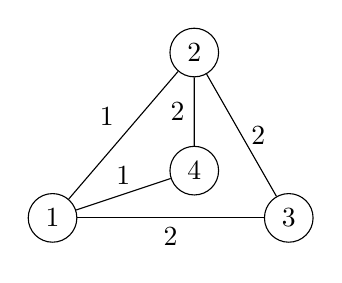
\begin{tikzpicture}[scale=0.6]
        \node[shape=circle,draw=black] (1) at (0,0) {1};
        \node[shape=circle,draw=black] (2) at (3,3.5) {2};
        \node[shape=circle,draw=black] (3) at (5,0) {3};
        \node[shape=circle,draw=black] (4) at (3,1) {4};

        \path [-] (1) edge node[above left] {$1$} (2); \path [-](2) edge
        node[right] {$2$} (3); \path [-](1) edge node[below] {$2$} (3); \path
        [-](2) edge node[left] {$2$} (4); \path [-](1) edge node[above] {$1$}
        (4);
    \end{tikzpicture}
    \captionof{figure}{Example of a weighted graph}
    \label{fig:weighted-graph-example}
\end{Figure}

The access to the graph are done via the \textit{adjacency list}.

\subsection{Graph Laplacian}
Let $G = (V, E, \omega)$ be a weighted graph, the Laplacian of $G$ is an $n
\times n$ matrix defined as
\begin{equation}
    L_G = D - A
\end{equation}
where $D$ is the degree matrix and $A$ is the adjacency matrix, defined
such that $(D)_{ii} = \sum_j \omega(i,j)$ and $(A)_{ij} = \omega(i,j)$. The
graph shown in Fig. \ref{fig:weighted-graph-example} has the following adjacency
and degree matrices
\begin{equation*}
    A = \begin{pmatrix}
        0 & 1 & 2 & 1 \\
        1 & 0 & 2 & 2 \\
        2 & 2 & 0 & 0 \\
        1 & 2 & 0 & 0 \\
    \end{pmatrix} \text{,} \;
    \quad
    D = \begin{pmatrix}
        4 & 0 & 0 & 0 \\
        0 & 5 & 0 & 0 \\
        0 & 0 & 4 & 0 \\
        0 & 0 & 0 & 3 \\
    \end{pmatrix} \text{,}
\end{equation*}
which yield the Laplacian
\begin{equation*}
    L = \begin{pmatrix}
        4 & -1 & -2 & -1 \\
        -1 & 5 & -2 & -2 \\
        -2 & -2 & 4 & 0 \\
        -1 & -2 & 0 & 3 \\
    \end{pmatrix} \text{.}
\end{equation*}

An interesting property of the Laplacian that arises from those definitions is
that $L_G$ is invertible if and only if the graph $G$ is connected.
Equivalently, the Laplacian of a graph can be expressed in terms of a weighted
sum of its edges Laplacian:
\begin{equation}
    L_Q = \sum_{(i,j)\in E} \omega(i,j)L_{(i,j)}
\end{equation}
where $L_{(i,j)}$ denotes the Laplacian of the edge $(i,j)$, defined as
\begin{equation}
    L_{(i,j)} = (\boldsymbol e_i - \boldsymbol e_j)(\boldsymbol e_i - \boldsymbol e_j)^T
\end{equation}
$\boldsymbol e_i$ is a unit vector with a 1 in coordinate $i$ and zeros
everywhere else. One can remark that $L_{(i,j)}$ is a very sparse matrix, with
only 4 nonzero entries.

% TODO : rephrase
The Laplacian is a positive semidefinite matrix i.e. the eigenvalues of the
Laplacian are non-negative.

% TODO : rephrase
The pseudo inverse of a Laplacian $L$ denoted $L^+$, is such that $LL^+L = L$
and $L^+LL^+ = L^+$.


\subsection{Quadratic forms of a Laplacian}
The quadratic form of a Laplacian has a number of nice properties, and can be
used to calculate quantities associated to the graph. All quadratic forms of a
Laplacian can be expressed, by linearity of the sum, in terms of a weighted sum
of its edges Laplacian:
\begin{equation}
    \begin{aligned}
        \x^T L_G \x
            & = \sum_{(i,j)\in E} \omega(i,j)\x^T L_{(i,j)}\x \\
            & = \sum_{(i,j)\in E} \omega(i,j)(\x(i) - \x(j))^2
    \end{aligned}
\end{equation}

An interesting example, showing how quadratic forms underlie graphs properties,
is that if $\x_s$ is an indicator vector on $S \subseteq V$, the quadratic form
$\x_s L_G \x_s$ is equal to the value of the cut $(S, S^c)$.

\subsection{Spectral Sparsification}

Spectral sparsification of graphs aims to reduce the number of edges, while
keeping an approximation of interesting quantities i.e., approximately preserving
all quadratic forms.

% TODO : maybe put the three equivalent definitions in the definition
% environement.
\begin{definition}[$\epsilon$-sparsifier]
    H is an $\epsilon$-sparsifier of G if and only if $\forall \x \in
    \mathbb{R}^n, \x^T L_H \x = (1 \pm \epsilon)\x^T L_G \x$.
\end{definition}

Using the pseudo-inverse of the Laplacian, this definition can be equivalently
formulated as $\x L_H^+ = (1 \pm O(\epsilon)) \x L_G^+\x$. It is also possible
to define an $\epsilon$-spectral sparsifier taking into account the positive
semidefinite property of the Laplacian, such that $(1-\epsilon) L_G \preccurlyeq
L_h \preccurlyeq (1+\epsilon) L_G$, where $\preccurlyeq$ denotes the partial
ordering on symmetric matrices. The three above definitions are equivalent and
one should use one or the other depending on the context.

\begin{theorem}[Graph Sparsifier]
    Every graph $G$ has an $\epsilon$-spectral sparsifier $H$ with a number of
    edges in $\tilde{O}(\frac{n}{\epsilon^2})$. Moreover, $H$ can be found in
    time $\tilde{O}(m)$.
\end{theorem}
One should note that this is relevant only when $\epsilon \leq \sqrt\frac{n}{m}$

The existence of such $\epsilon$-spectral sparsifier was proved by Spielman and
Teng \cite{spielman_spectral_2011}. Additional work of Batson, Spielman
and Strivastava \cite{batson_twice-ramanujan_2012} reduced the lower bound on the
number of edges in the sparsifier to $O(\frac{n}{\epsilon ^2})$.


% \subsection{Applications}